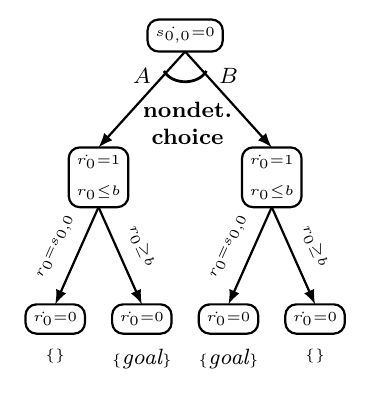
\begin{tikzpicture}[
    %scale=0.1,
    %framed,
    grow=down,
    level 1/.style={sibling distance=2.2cm,level distance=1.8cm},
    level 2/.style={sibling distance=1.1cm, level distance=1.8cm},
    %level 3/.style={sibling distance=1cm, level distance=1.5cm},
    edge from parent/.style={thick,draw=black, ->, >=latex},
    edge from parent path={(\tikzparentnode.south) -- (\tikzchildnode.north)},
    kant/.style={text width=2cm, text centered}, %sloped
    every node/.style={text ragged, inner sep=2mm, outer sep=0cm, font=\footnotesize},
    punkt/.style={inner sep=1mm, rectangle, rounded corners, draw=black, thick, font=\small }
    ]
    \useasboundingbox (-2,0.1) rectangle (2,-4.2);
\node[punkt][rectangle] {$\scriptscriptstyle\dot{s_{0,0}} = 0$}
    child {
        node[punkt, align=center] {$\scriptscriptstyle\dot{r_0} = 1$\\$\scriptscriptstyle r_0\leq b$}
            child {
                node[punkt, label={below:\footnotesize $\scriptscriptstyle\{\}$}] {$\scriptscriptstyle\dot{r_0} = 0$} % no goal
            edge from parent
                node[sloped, kant, above, pos=.5] {\footnotesize $\scriptscriptstyle r_0=s_{0,0}$}
            }
            child {
                node[punkt, label={below:\footnotesize $\scriptscriptstyle\{\textit{goal}\}$}] {$\scriptscriptstyle\dot{r_0} = 0$} % goal
            edge from parent
                node[sloped, kant, above, pos=.5] {\footnotesize $\scriptscriptstyle r_0\geq b$}
            }
        edge from parent
                node[kant, above] {$A$}
    }
    child {
        node[punkt, align=center] {$\scriptscriptstyle\dot{r_0} = 1$\\$\scriptscriptstyle r_0\leq b$}
            child {
                node[punkt, label={below:\footnotesize $\scriptscriptstyle\{\textit{goal}\}$}] {$\scriptscriptstyle\dot{r_0} = 0$} % goal
            edge from parent
                node[sloped, kant, above, pos=.5] {\footnotesize $\scriptscriptstyle r_0=s_{0,0}$}
            }
            child {
                node[punkt, label={below:\footnotesize $\scriptscriptstyle\{\}$}] {$\scriptscriptstyle\dot{r_0} = 0$} % no goal
            edge from parent
                node[sloped, kant, above, pos=.5] {\footnotesize $\scriptscriptstyle r_0\geq b$}
            }
        edge from parent
                node[kant, above] {$B$}
    };


\draw [-,line width=1pt] (0.27,-0.45) to[bend left=60,looseness=1] (-0.27,-0.45) node[below, xshift=0.3cm, yshift=-0.2cm,align=center] {\footnotesize\textbf{nondet.} \\\footnotesize \textbf{choice}};
\end{tikzpicture}
